% Working manuscript name. Rename to the assigned IBIC2026 programme code.
\documentclass[]{jacow}

\usepackage[english]{babel}
\usepackage{booktabs}
\usepackage{graphicx}
\usepackage{siunitx}

\newcommand{\qhat}{\widehat{q}}
\newcommand{\bestn}{Best-$N$}
% Generated by scripts/prepare_ibic2026_publication.py; do not edit.
\newcommand{\PrimaryHBestOneScore}{0.343}
\newcommand{\PrimaryHBestThreeScore}{0.392}
\newcommand{\PrimaryHBestFiveScore}{0.403}
\newcommand{\PrimaryVBestOneScore}{0.420}
\newcommand{\PrimaryVBestThreeScore}{0.484}
\newcommand{\PrimaryVBestFiveScore}{0.524}
\newcommand{\PrimaryHOneToThreeGain}{0.0500}
\newcommand{\PrimaryHThreeToFiveGain}{0.0122}
\newcommand{\PrimaryVOneToThreeGain}{0.0646}
\newcommand{\PrimaryVThreeToFiveGain}{0.0310}
\newcommand{\IntensityEffectCount}{240}
\newcommand{\IntensityFdrCount}{0}
\newcommand{\IntensityPracticalCount}{0}
\newcommand{\IntensityRetainedCount}{0}
\newcommand{\BestNCurveSpillPlaneCount}{4000}
\newcommand{\BestNValidationSpillPlaneCount}{1000}
\newcommand{\BestNDigitizerFoldCount}{5}
\newcommand{\BestNHSensitivityAvailable}{5}
\newcommand{\BestNHSensitivityUnavailable}{2}
\newcommand{\BestNHSensitivityMinimum}{2}
\newcommand{\BestNHSensitivityMaximum}{13}
\newcommand{\BestNVSensitivityAvailable}{6}
\newcommand{\BestNVSensitivityUnavailable}{1}
\newcommand{\BestNVSensitivityMinimum}{10}
\newcommand{\BestNVSensitivityMaximum}{28}
\newcommand{\AllTrainingHSelectedFavored}{2}
\newcommand{\AllTrainingHBaselineFavored}{3}
\newcommand{\AllTrainingHUnresolved}{3}
\newcommand{\AllTrainingVSelectedFavored}{3}
\newcommand{\AllTrainingVBaselineFavored}{3}
\newcommand{\AllTrainingVUnresolved}{2}
\newcommand{\RidgeHStructuralRows}{360000}
\newcommand{\RidgeHFinitePicks}{359018}
\newcommand{\RidgeHBlankPicks}{14}
\newcommand{\RidgeHEdgeExcludedPicks}{968}
\newcommand{\RidgeVStructuralRows}{360000}
\newcommand{\RidgeVFinitePicks}{289210}
\newcommand{\RidgeVBlankPicks}{69684}
\newcommand{\RidgeVEdgeExcludedPicks}{1106}
\newcommand{\PrimarySpillCount}{2000}
\newcommand{\PrimaryNominalHChannels}{60}
\newcommand{\PrimaryNominalVChannels}{60}
\newcommand{\PrimaryPartialCaptures}{12}
\newcommand{\PrimarySourceAbsences}{16}


\begin{document}

\title{Turn-by-turn tune analysis using adaptive \NoCaseChange{BPM} ensembles in the Fermilab \NoCaseChange{Mu2e} Delivery Ring\thanks{This manuscript has been authored by Fermi Forward Discovery Group, LLC under Contract No. 89243024CSC000002 with the U.S. Department of Energy, Office of Science, Office of High Energy Physics.}}

\author[1]{D. Steinkamp\thanks{derekste@fnal.gov}}
\affil[1]{Fermi National Accelerator Laboratory, Batavia, Illinois, USA}

\maketitle

\begin{abstract}
The Mu2e experiment at Fermilab requires stable resonant slow extraction from the Delivery Ring, making reliable tune monitoring an important operational diagnostic. This work investigates BPM-based tune-candidate extraction using synchronized turn-by-turn position data distributed across multiple digitizers. Each spill contains approximately 50,000 turns from many BPMs in both transverse planes, enabling spectral analysis of tune-like structure.

The analysis captures coherent spill snapshots, verifies synchronization using stream timestamps, and computes tune candidates in configurable horizontal and vertical tune bands. Rather than relying on a single BPM or fixed BPM list, it evaluates BPM quality on a spill-by-spill basis and selects small adaptive BPM ensembles. A multi-spill study shows that tune observability is distributed and dynamic rather than concentrated in one globally optimal BPM. Adaptive ensembles improve tune-candidate quality compared with single-BPM selections, with the clearest results in the vertical plane. The horizontal plane shows useful ranking structure but weaker visibility under present thresholds.

Direct evaluation of fixed global BPM sets shows that static selections do not reproduce dynamic per-spill performance. These results motivate an adaptive BPM-ensemble approach for Delivery Ring tune analysis using selected BPM subsets, confidence metrics, and quality flags rather than a single preferred BPM or fixed BPM list.
\end{abstract}

\section{Introduction}

The Mu2e slow-extraction programme uses third-integer resonant extraction from the Fermilab Delivery Ring. Spill regulation depends on a tune-ramp quadrupole family and radio-frequency knock-out excitation, making transverse tune observability relevant to both commissioning and operations~\cite{ibrahim:ibic2019-mopp033,nagaslaev:prab2019,nagaslaev:commissioning2026}. The installed Muon Campus BPM system provides synchronized turn-by-turn (TBT) position waveforms throughout the ring~\cite{patel:ibic2019-wepp044}. A single BPM, however, need not remain the best observer as orbit, oscillation amplitude, extraction conditions, and instrument quality change.

Combining TBT data from multiple BPMs can improve tune estimation when individual signals have unequal signal-to-noise ratio or decohere rapidly~\cite{zisopoulos:ipac2017-mopab122,alexahin:ipac2010-mope084}. The central question here is therefore not which BPM is globally best, but how many BPMs should be combined for each spill and whether that adaptive choice is reproducible outside the data used to make it.

This paper reports a BPM-only internal validation. The reported values are fractional tune candidates in configured search bands. No Schottky, tune-meter, or controlled tune-knob reference was available for these captures, so the analysis does not claim absolute tune accuracy.

\section{Data and synchronization}

The primary data set contains 2,000 captured spills in two acquisition collections. Each usable spill supplies 60 horizontal and 60 vertical position channels, with two same-plane source channels per digitizer, and approximately 50,000 turns per channel. Stream timestamps are used to assemble a coherent spill snapshot. Adjacent target buckets are merged within \qty{1}{ms}, while captured streams are checked against the selected target using the separately configured \qty{25}{ms} same-spill tolerance. Incomplete or inconsistent states carry quality flags rather than being silently accepted.

Publication auditing exposed two identity defects in an earlier analysis. First, downstream tables stored a shared digitizer label rather than the exact channel key, even though two same-plane channels could share that label. Second, ring order was parsed from the first number in the digitizer address, assigning every channel the same order and disabling the intended ring-span term. The corrected pipeline serializes plane-local indices, exact BPM tokens, full source keys, and digitizer identities. Every downstream reconstruction resolves the subset bit mask before display labels.

The waveform path subtracts the window mean, applies a Hann taper, and computes a zero-padded real fast Fourier transform. Frequencies are mapped to the upper fractional tune branch by $q=1-f$. The discovery bands are $0.60\leq q_x\leq0.70$ and $0.67\leq q_y\leq0.75$; expected values near 0.65 and 0.72 enter only as soft priors.

\section{Adaptive ensemble method}

For the primary search, overlapping 4,096-turn windows with 256-turn stride characterize early-spill spectral structure. Per-BPM peak candidates are clustered within each spill and plane to form an internal consensus; no distribution across other spills is used as a label. Candidate subset spectra are averaged in power. The score combines held-out channel support, robust peak prominence and entropy, agreement with the within-spill consensus, window stability, visibility, digitizer and ring diversity, and an ambiguity penalty. Turn-dependent diagnostics are retained because extraction records are nonstationary~\cite{russo:prab2024}.

Best-1 and Best-3 are searched exhaustively over the 60 channels in a plane. Best-5 uses exhaustive enumeration within a recorded 20-channel screening pool. Because the score is a model-selection statistic rather than a measurement uncertainty, all publication claims are checked in the independent protocol below.

\subsection{Leakage-controlled \bestn{} selection}

The ensemble-size study sweeps contiguous $N$ values instead of comparing only 1, 3, and 5. Members are selected from a prefix of eight fit windows. Every later window overlapping that prefix is purged; evaluation begins at the first non-overlapping window. Candidate tunes are derived only from fit windows.

The full $N$ curve uses \BestNCurveSpillPlaneCount{} spill-plane cases; digitizer-disjoint validation uses an evenly stratified \BestNValidationSpillPlaneCount{}-case subset, each evaluated across \BestNDigitizerFoldCount{} folds rather than being presented as the full curve population.

A bounded beam search is used above $N=1$ and is repeated at multiple beam widths. Convergence is judged from membership, score, and tune differences, not membership alone. For channel-disjoint validation, complete digitizers are assigned to folds so sibling channels never appear on opposite sides. Each fold selects from the training digitizers and is evaluated on later windows; the reference is a median-power spectrum from held-out digitizers.

Two agreement measures are retained. The conditioned measure searches near the training tune and answers whether later spectra support that candidate. The blind measure searches the full configured band independently for selected and held-out channels. The smallest non-inferior $N$ is chosen only after blind agreement and channel-disjoint tune difference are screened, followed by both selected-channel and held-out-channel power support and prominence. Confidence intervals collapse folds within a spill and use a moving-block bootstrap within each capture collection to retain short-range serial dependence. As a final hyperparameter check, $N$ is chosen from one acquisition collection and the same global $N$ is evaluated in the other; only the per-spill members remain adaptive.

\section{Results}

\subsection{Corrected adaptive search}

Across 4,000 corrected spill-plane rows per subset size, the median adaptive-search score rises from \PrimaryHBestOneScore{} to \PrimaryHBestThreeScore{} and \PrimaryHBestFiveScore{} for horizontal Best-1, Best-3, and Best-5, and from \PrimaryVBestOneScore{} to \PrimaryVBestThreeScore{} and \PrimaryVBestFiveScore{} vertically. Paired Best-1-to-Best-3 gains are \PrimaryHOneToThreeGain{} horizontally and \PrimaryVOneToThreeGain{} vertically; Best-3-to-Best-5 gains are \PrimaryHThreeToFiveGain{} and \PrimaryVThreeToFiveGain{}. These are in-sample model-selection scores, not tune-accuracy measurements. Leakage-controlled later-window results and exact-paired persistence metrics are reported in Table~\ref{tab:results}.

Across seven verified reduced-sample beam, fit-window, and fold-seed checks, eligible H knees span Best-\BestNHSensitivityMinimum{}--Best-\BestNHSensitivityMaximum{} in \BestNHSensitivityAvailable{}/7 runs, with \BestNHSensitivityUnavailable{} unresolved; V spans Best-\BestNVSensitivityMinimum{}--Best-\BestNVSensitivityMaximum{} in \BestNVSensitivityAvailable{}/7, with \BestNVSensitivityUnavailable{} unresolved. Unresolved cases are retained as sensitivity evidence rather than coerced into a recommendation; the full-data selections drive the persistence figures.

\IfFileExists{figures/best_n_validation_h.png}{%
\begin{figure*}[!htb]
  \centering
  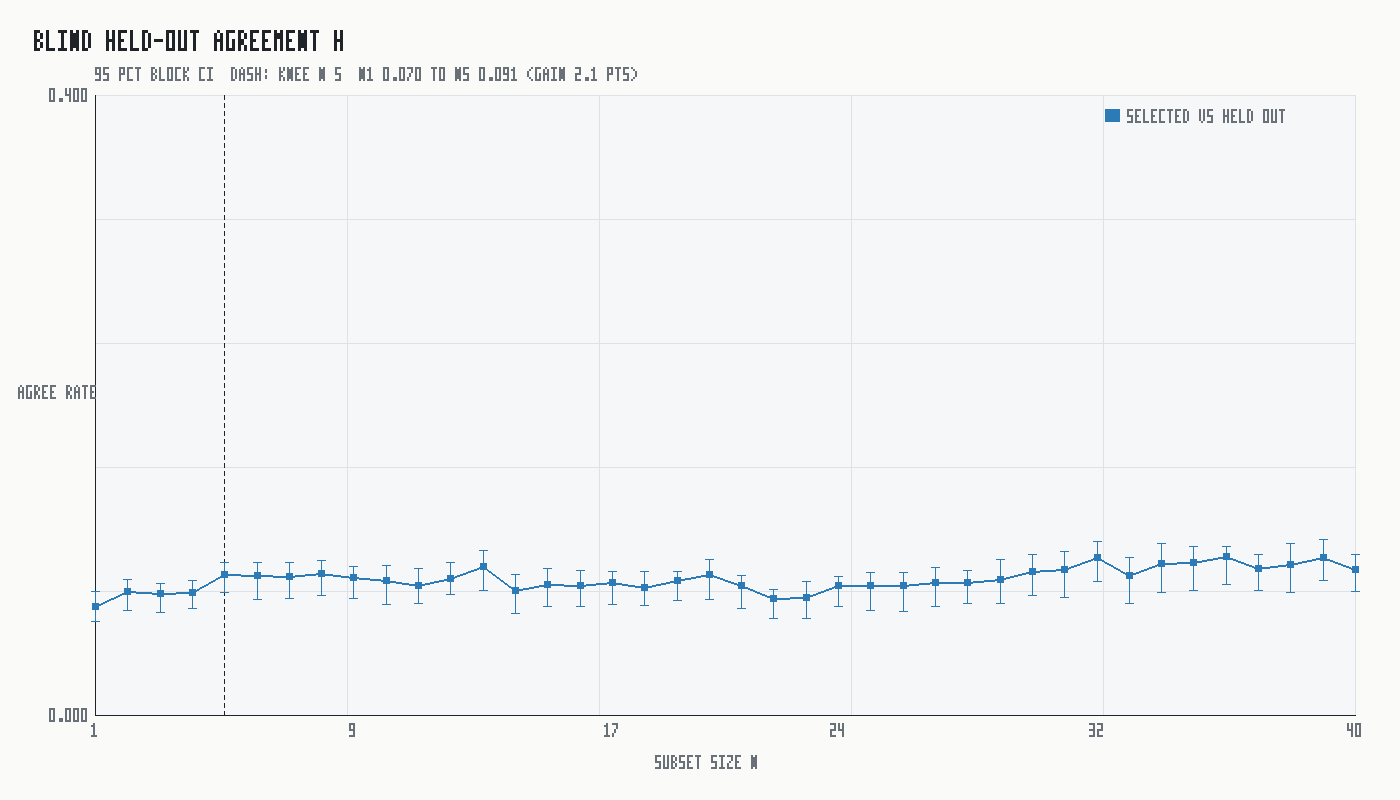
\includegraphics[width=0.49\textwidth]{figures/best_n_validation_h.png}\hfill
  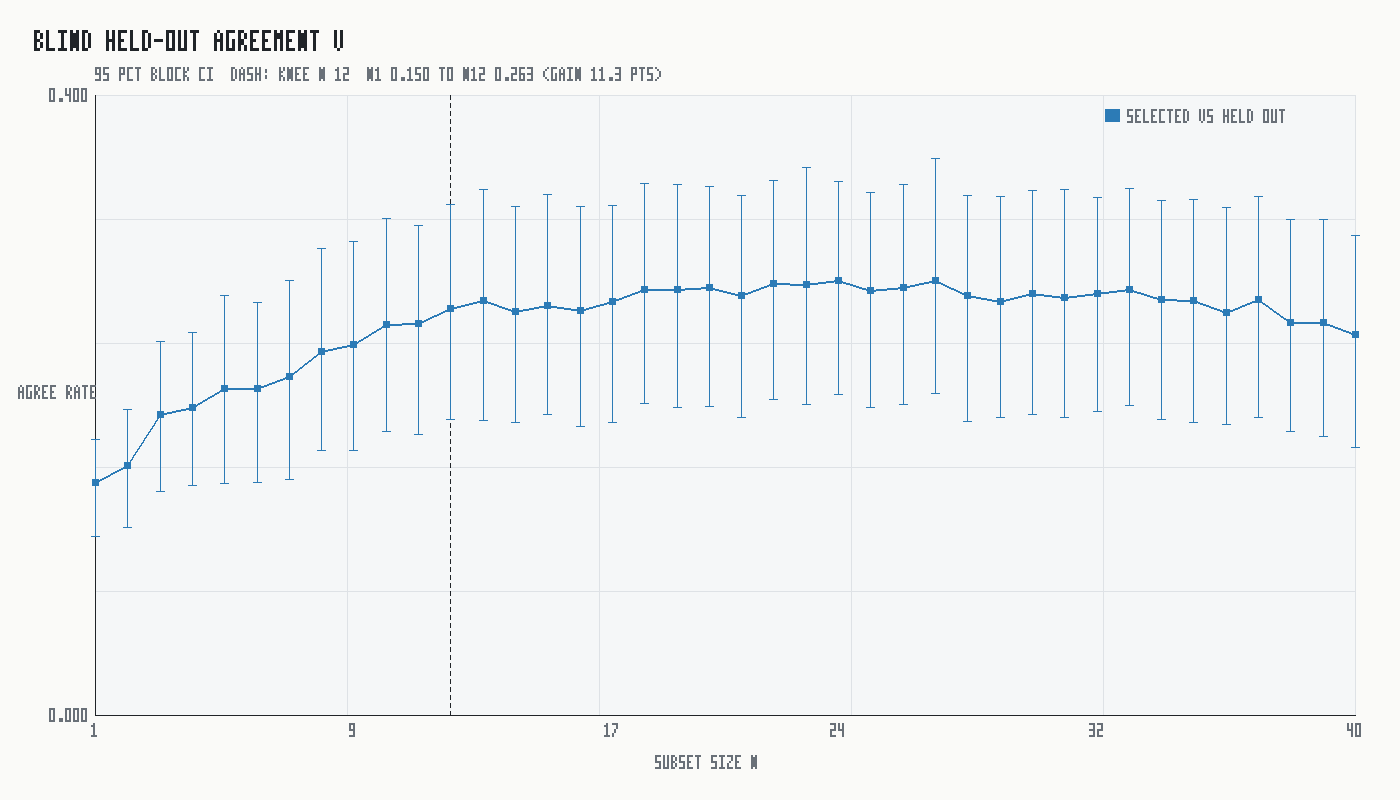
\includegraphics[width=0.49\textwidth]{figures/best_n_validation_v.png}
  \caption{Leakage-controlled \bestn{} validation for the horizontal (left) and vertical (right) planes. Blind full-band selected-versus-held-out digitizer agreement is shown with moving-block intervals; conditioned support near the fitted candidate is reported separately.}
  \label{fig:bestn}
\end{figure*}
}{}

\IfFileExists{results_table.tex}{\begin{table*}[!htb]
  \centering
  \caption{Leakage-controlled Best-$N$ intervals use collection-preserving spill blocks. Ridge intervals use overlapping-turn blocks on exact-paired picks and describe concentration, not absolute tune accuracy or measured physical noise.}
  \label{tab:results}
  \small
  \begin{tabular}{@{}lcccc@{}}
    \toprule
    Plane & Best-$N$ & Blind agreement (\%) & Blind $|\Delta q|$ ($10^{-3}$) & $\Delta$IQR vs B1 ($10^{-3}$) \\
    \midrule
    H & 5 & 9.1 [7.9, 9.8] & 16.1 [15.5, 17.2] & -2.4 [-3.1, -1.9] \\
    V & 12 & 26.3 [19.1, 33.0] & 10.7 [9.7, 12.0] & 1.0 [0.4, 1.7] \\
    \bottomrule
  \end{tabular}
\end{table*}
}{}

\subsection{Full-spill ridge-density comparison}

To visualize persistence through the approximately 50,000-turn record, the selected early-window membership is applied to the raw captured spill. Each selected trace is RMS-normalized, 4,096-turn Hann spectra are computed every 256 turns, and selected-BPM powers are averaged. One locally tracked ridge pick per spill and window is binned across spills. This plot is a density of selected ridge locations, not a spectral-power heat map.

The legacy comparator uses identical tune bands and binning but came from a normalized single-channel selector whose winner was effectively determined by floating-point residuals after RMS normalization. It is therefore labeled ``legacy normalized-single'', not ``best BPM''. Paired panels use exact common spill/window ridge points and one color scale. Difference maps subtract column-normalized ridge-pick densities; they quantify redistribution and concentration of ridge picks, not physical noise removal. A separate corrected-Best-1 comparison isolates ensemble size from repair of that historical selector. Moving-block intervals across turn centers test whether paired concentration changes persist despite the heavily overlapping windows; they are not uncertainty estimates over the spill population.

\IfFileExists{figures/ridge_density_comparison.png}{%
\begin{figure*}[!htb]
  \centering
  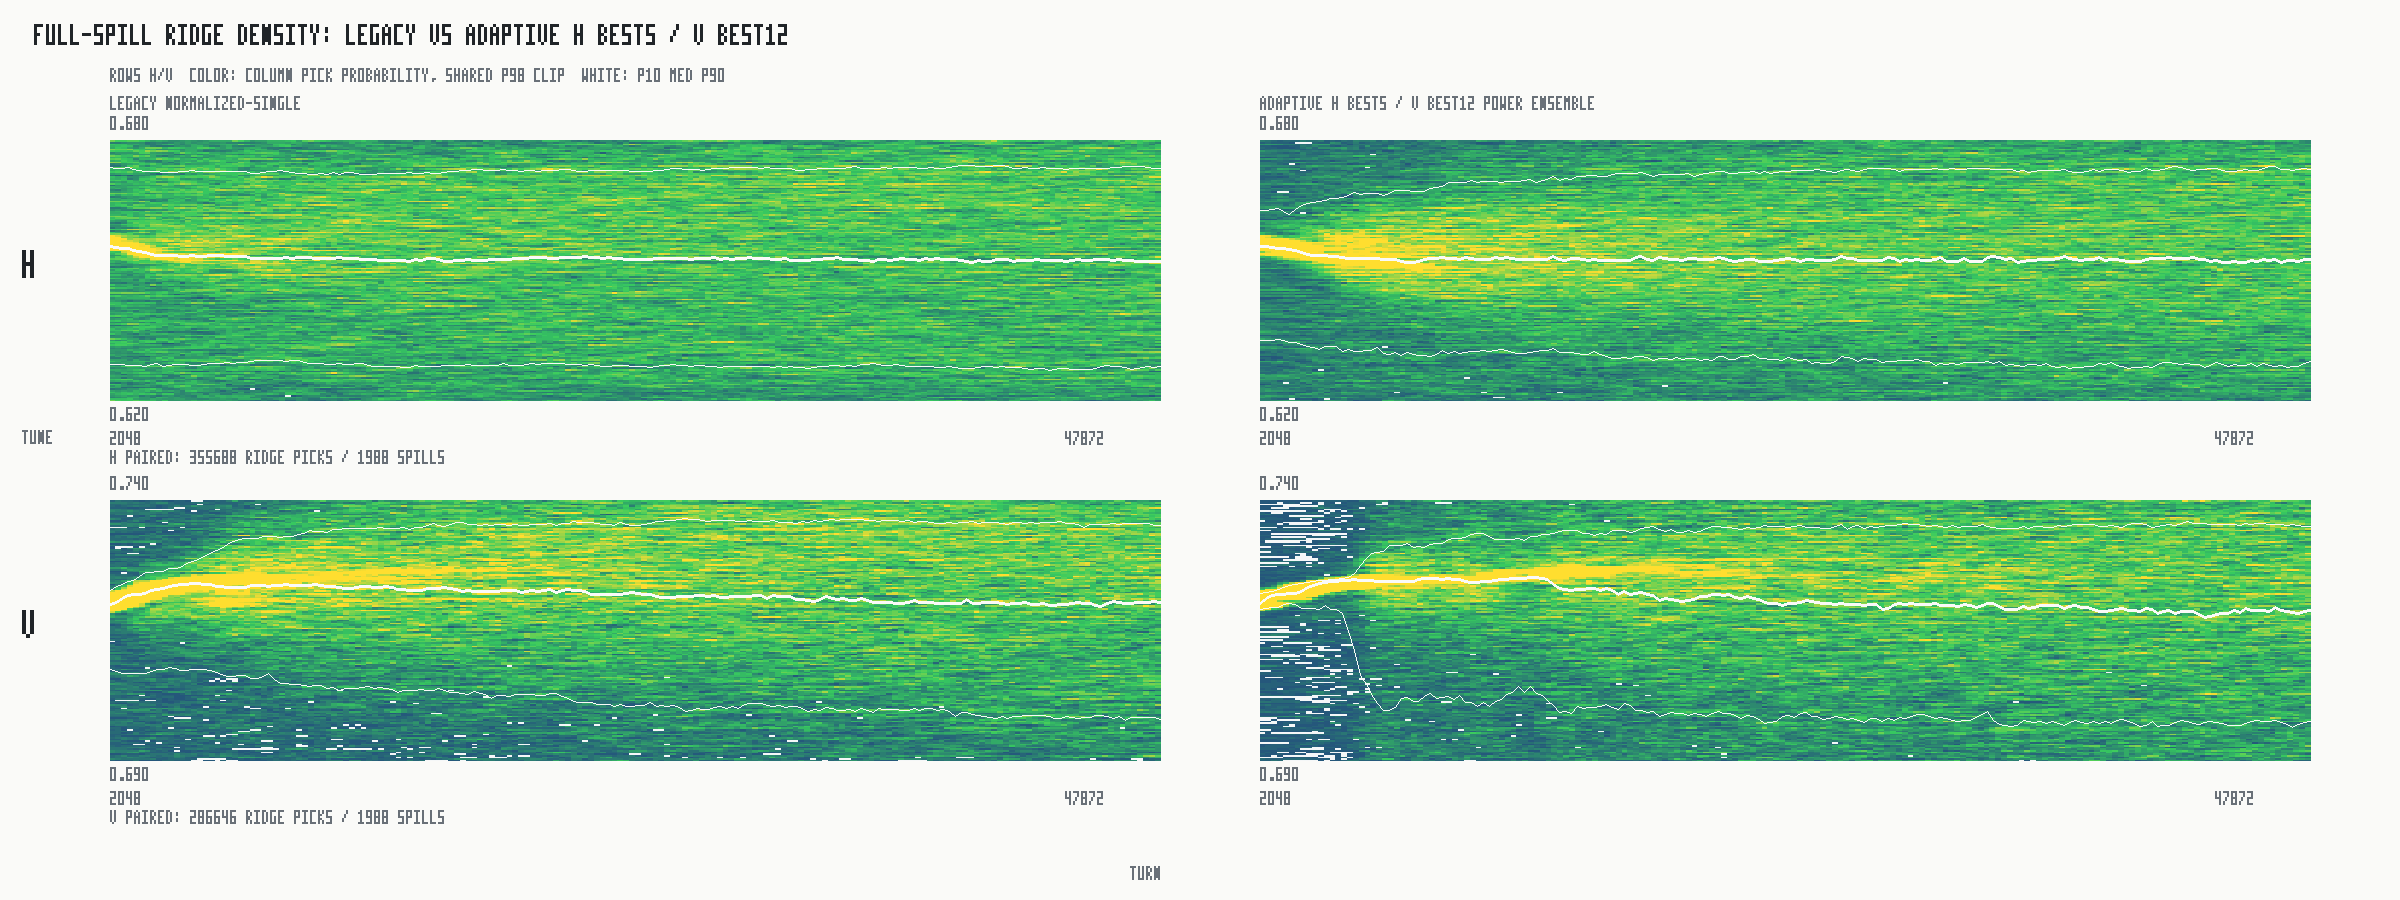
\includegraphics[width=0.98\textwidth]{figures/ridge_density_comparison.png}
  \caption{Full-spill ridge-pick density for the legacy normalized-single method and the selected adaptive ensemble on exact common spill/window points. Color is column-normalized cross-spill pick probability with one shared P98-clipped scale; white curves show cross-spill P10, median, and P90 tracks. Horizontal and vertical results are interpreted separately.}
  \label{fig:ridge}
\end{figure*}
}{}

\IfFileExists{figures/ridge_width_contrast_hv.png}{%
\begin{figure*}[!htb]
  \centering
  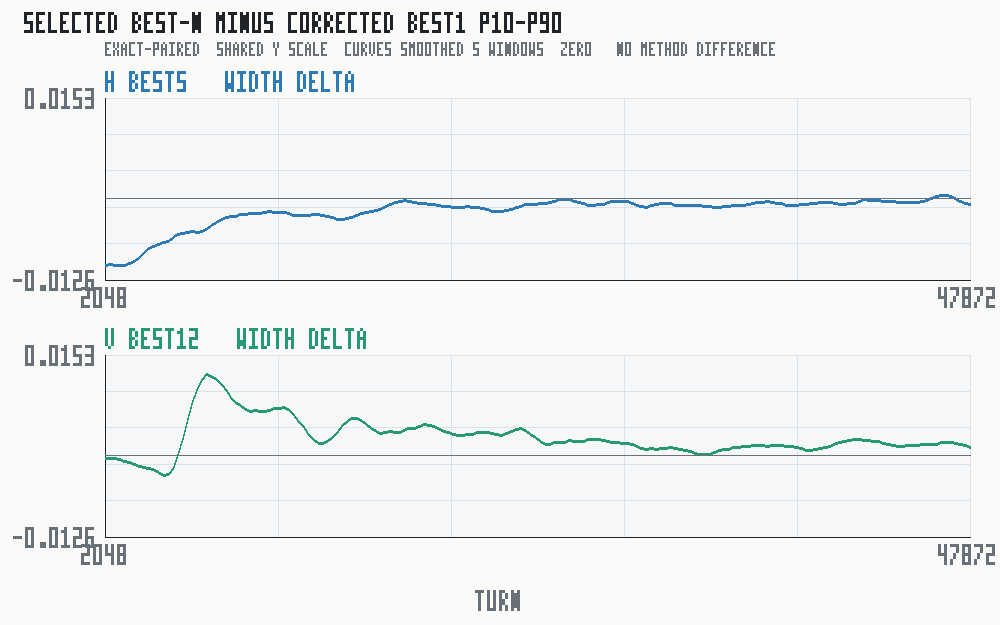
\includegraphics[width=0.94\textwidth]{figures/ridge_width_contrast_hv.png}
  \caption{Exact-paired selected-Best-$N$ minus corrected-Best-1 P10--P90 ridge-pick width for the horizontal and vertical planes. Negative values indicate a narrower selected-ensemble cross-spill pick distribution at that turn center. Both panels use one y scale. Exported values are unsmoothed; the curves use five-window visual smoothing. This isolates ensemble size under the fixed protocol but does not establish physical noise removal, absolute tune accuracy, or extraction timing.}
  \label{fig:ridgewidth}
\end{figure*}
}{}

\subsection{Fixed sets, intensity, and plane asymmetry}

Frozen global top-1, top-3, and top-5 sets are trained on one acquisition collection and applied to the other. Dynamic memberships, frozen memberships, and all-BPM controls are rescored from the same cached spectra with one evolution metric. This comparison is descriptive because the original dynamic memberships reuse selection windows; the corrected result is reported alongside the leakage-controlled Best-N inference rather than used as an independent validation test.

A separate 200-spill capture supplies 23,999 exact raw position/intensity channel pairs; one expected pair is absent. For the pairs present, the first 50,000 turns pass the structural checks, while advertised longer arrays become unreliable near turn 64,000 and are excluded. Square-root, linear, and gated intensity weights are compared with unweighted spectral aggregation on purged later windows. A window with no usable selected intensity falls back explicitly to unweighted aggregation, and the $N=1$ case is an exact zero-effect control. Across \IntensityEffectCount{} paired method-effect tests, a 20-spill moving-block bootstrap and block sign-flip test leave \IntensityFdrCount{} false-discovery-rate-significant directional effects within tune tolerance, \IntensityPracticalCount{} effects above the declared practical thresholds, and \IntensityRetainedCount{} retained weighting effects. Intensity is therefore retained as an envelope and integrity diagnostic rather than a tune weight.

The vertical plane gives the clearest sustained, channel-disjoint structure. Horizontal rankings improve with adaptive selection, but visibility decays or becomes diffuse earlier and more variably. No fixed extraction-onset turn is imposed: the machine onset can vary, and a previously suggested 10,000--20,000-turn interval is treated only as review context. Horizontal loss diagnostics therefore report turn-dependent concentration and data-derived sustained-loss points without assigning cause.

\IfFileExists{figures/horizontal_loss_diagnostic.png}{%
\begin{figure}[!htb]
  \centering
  
\includegraphics[width=0.98\columnwidth]{figures/horizontal_loss_diagnostic.png}
  \caption{Horizontal ridge-concentration diagnostic over the full record. The loss candidate is derived from sustained changes in concentration and retained-spill fraction; the broad extraction-review interval is not used to choose it and no causal mechanism is assigned.}
  \label{fig:hloss}
\end{figure}
}{}

\section{Limitations and operational use}

The study has four principal limits. First, internal BPM agreement is not an independent tune calibration. Second, captures span unlabeled machine states; block-aware uncertainty does not replace controlled scans. Third, early-window membership is held fixed in the 50,000-turn visualization, so that figure tests persistence rather than full-spill reselection. Fourth, ridge-density concentration can improve even if all methods follow the same biased candidate. These limits motivate a future matched Schottky or tune-meter comparison and controlled tune-knob study.

Within those limits, adaptive ensembles are operationally preferable to a single preferred BPM or static list. A practical monitor should expose the selected exact channels, ensemble size, tune candidate, prominence and ambiguity measures, later-window support, and a no-reliable-tune state. Horizontal and vertical quality decisions should remain independent.

\section{Conclusion}

Synchronized distributed BPM streams can recover repeatable tune-like spectral structure when small ensembles are selected spill by spill. Leakage-controlled, digitizer-disjoint validation determines the useful ensemble size rather than assuming that more BPMs are better. The strongest result is vertical; the horizontal plane remains a diagnostic limitation rather than a symmetric claim. Fixed global sets and intensity weighting do not replace adaptive position-channel selection. The method is therefore a defensible BPM-only tune-candidate diagnostic and a foundation for later externally calibrated tune monitoring.

\begin{thebibliography}{9}

\bibitem{ibrahim:ibic2019-mopp033}
M. A. Ibrahim \textit{et al.}, ``Preliminary design of Mu2E Spill Regulation System (SRS)'', in \textit{Proc. IBIC'19}, Malm\"o, Sweden, Sep. 2019, paper MOPP033, pp.~177--180. \doi{10.18429/JACoW-IBIC2019-MOPP033}

\bibitem{nagaslaev:prab2019}
V. Nagaslaev, K. A. Brown, and M. Tomizawa, ``Third integer resonance extraction with presence of higher multipoles'', \textit{Phys. Rev. Accel. Beams}, vol.~22, p.~043501, 2019. \doi{10.1103/PhysRevAccelBeams.22.043501}

\bibitem{nagaslaev:commissioning2026}
V. Nagaslaev \textit{et al.}, ``Slow extraction beam commissioning for the Mu2e experiment at Fermilab'', 2026. \doi{10.48550/arXiv.2606.25140}

\bibitem{patel:ibic2019-wepp044}
N. Patel \textit{et al.}, ``Beam position monitoring system for Fermilab's Muon Campus'', in \textit{Proc. IBIC'19}, Malm\"o, Sweden, Sep. 2019, paper WEPP044, pp.~648--650. \doi{10.18429/JACoW-IBIC2019-WEPP044}

\bibitem{zisopoulos:ipac2017-mopab122}
P. Zisopoulos, M. G\k{a}sior, M. Serluca, and G. Sterbini, ``Fast bunch by bunch tune measurements at the CERN PS'', in \textit{Proc. IPAC'17}, Copenhagen, Denmark, May 2017, paper MOPAB122, pp.~415--418. \doi{10.18429/JACoW-IPAC2017-MOPAB122}

\bibitem{alexahin:ipac2010-mope084}
Y. Alexahin, E. Gianfelice-Wendt, and W. L. Marsh, ``Tune evaluation from phased BPM turn-by-turn data'', in \textit{Proc. IPAC'10}, Kyoto, Japan, May 2010, paper MOPE084, pp.~1179--1181.

\bibitem{russo:prab2024}
G. Russo, G. Franchetti, M. Giovannozzi, and E. H. Maclean, ``Harmonic analysis of nonstationary signals with application to LHC beam measurements'', \textit{Phys. Rev. Accel. Beams}, vol.~27, p.~094001, 2024. \doi{10.1103/PhysRevAccelBeams.27.094001}

\end{thebibliography}

\end{document}
